% вторая часть

\section{Аппаратная часть}
\subsection{Обзор аппаратно-программного комплекса «СКАУТ»}
Обычно, жилой дом становится умным, благодаря применению в нем аппаратно-программного комплекса СКАУТ. Задача СКАУТА --- усиление безопасности, экономия ресурсов и повышение комфорта жителей. \cite{Almanah}

Функции аппаратно-программного комплекса СКАУТ можно разделить на семь, тесно связанных между собой, систем.
\begin{enumerate}
	\item Контроль доступа; 
	\item Учет ресурсов;
	\item Оповещение;
	\item Wi-Fi;
	\item Охрана технических помещений;
	\item Управление оборудованием;
	\item Видеонаблюдение.
\end{enumerate} 

Для доступа или въезда на территорию комплекса используется универсальный электронный ключ. Ключ является персональным для жителей, его копирование или подделка исключена. Все технические помещения находятся под контролем скаута. Снятие и постановка на охрану осуществляется техническим персоналом самостоятельно, с помощью мобильного телефона. Универсальный механический ключ удобен в эксплуатации и облегчает перемещение работников. 

Все потребляемые жителями ресурсы полностью учитываются и публикуются на сайте управляющей компании. Автоматизированный анализ показаний позволяет своевременно выявлять нарушении режимов отопления, неисправности приборов учета, возникающие аварии. 

Громкоговорящая система оповещения и информирования вовремя предупредит о планируемых ремонтных работах, причинах и сроках ликвидации аварийных ситуаций. Оператору управляющей компанией достаточно набрать текст сообщения и очертить на электронной карте зону оповещения. 

В чрезвычайных ситуациях диспетчер управляющей компании в ручном режиме может управлять электрооборудованием дома: шлагбаумами, электрозадвижками, системой дымоудаления, пожарными насосами.

Система видеонаблюдения, кроме охранных функций, осуществляет контроль исполнения команд диспетчера. Дает информацию о заполненности парковки на мобильные устройства. Система видеонаблюдения включена в муниципальный комплекс Безопасный город.

Используя Wi-Fi технологию, СКАУТ обеспечивает работникам управляющей компанией мобильный доступ к проектной документации, связь с диспетчером, передачу контрольной и видео информаций в аварийных случаях. 

Каждый житель цифрового района имеет доступ к данным системам СКАУТ через личный кабинет, в котором может получить видеоинформацию, организовать доступ гостей и родственников, получить информацию по коммунальным платежам. 

Умный город состоит из умных домов, а пока СКАУТ ступень к новому качеству жизни.

\subsection{Raspberry Pi 2 model B}

Благодаря своему небольшому размеру, малой стоимости, хорошей вычислительной мощности и качественной поддержке со стороны производителя в качестве главной вычислительной мощности был выбран одноплатный миникомпьютер фирмы Raspberry Pi. 

\subsubsection{Описание}

Raspberry Pi - миниатюрный одноплатный компьютер изображен на рисунке~\ref{fig:raspberry}. \cite{Raspberry} Из-за широкой функциональности и небольшой стоимости Raspberry Pi получил широкое распространение среди разработчиков и любителей электроники. Данный компьютер обладает следующими преимуществами:

\begin{itemize}
	\item Малый размер, 85,6 x 54,0 x 17 мм;
	\item Вычислительная мощность;
	\item Удобный софт и техподдержка;
	\item Малая стоимость, около 35 \$;
	\item Потребляемая мощность меньше 10 Вт;
\end{itemize}

\begin{figure}[H]
	\centering
	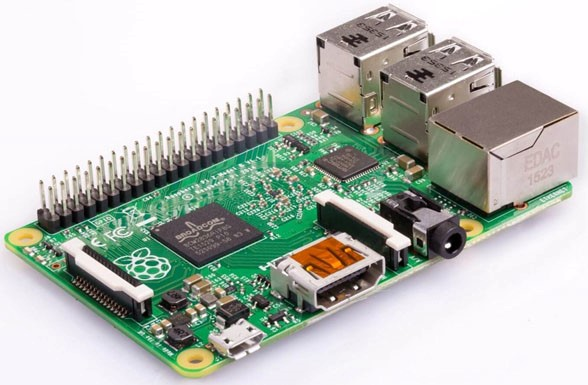
\includegraphics[width=0.7\linewidth]{pics/raspberry}
	\caption{Raspberry Pi 2 model B}
	\label{fig:raspberry} 
\end{figure}

\subsubsection{Технические характеристики}
Рассмотрим технические характеристики в таблице~\ref{tab:tab2}
\begin{table}[H]
	\caption{Технические характеристики Raspberry Pi 2 model B} \label{tab:tab2}
	\centering
	\begin{tabular}{|p{3.5cm}|p{12cm}|}
		\hline
		\multicolumn{2}{|c|}{Технические характеристики} \\
		\hline 
		Система на кристалле (SoC) & Broadcom BCM2836 (CPU + GPU) \\ 
		\hline 
		Процессор & 32-битный четырехъядерный ARMv7-A Cortex-A7 с тактовой частотой 900 МГц, 16 КБ cache L1 и 256 КБ cache L2 \\ 
		Графический процессор & Двухъядерный процессор (GPU) VideoCore IV® с тактовой частотой 250 МГц поддерживает стандарты OpenGL ES 2.0, OpenVG, MPEG-2, VC-1 и способен кодировать, декодировать и выводить Full HD-видео (1080p, 30 FPS, H.264 High-Profil) \\ 
		\hline 
		ОЗУ & 1 ГБ SDRAM LPDDR2 900 МГц EDB8132B4PB-8D-F (совместно с GPU) \\ 
		\hline 
		Хранилище & слот для карты памяти MicroSDHC, USB Boot Mode \\ 
		\hline 
		Ethernet & 10/100 Мбит с выходом на стандартное гнездо 8P8C (RJ45) (контроллер LAN9514-JZX — USB 2.0 Hub и 10/100 Ethernet) \\ 
		\hline 
		Видео вход & 1 x CSI-2 для подключения камеры по интерфейсу MIPI \\ 
		\hline 
		Видео выход & 1 x HDMI 1.3a (CEC) 1 x DSI (Display Serial Interface) для подключения штатного дисплея; 1 x композитный видеовыход (CVBS видео, PAL и NTSC) 3.5 мм разъем \\ 
		\hline 
		Аудио вход & I$^{2}$S \\ 
		\hline 
		Аудио выход & гнездо 3.5 мм, HDMI \\ 
		\hline 
		USB-порты & 4 порта USB 2.0 через USB hub в LAN9514-JZX \\ 
		\hline 
		Периферия & 40 портов ввода-вывода общего назначения (GPIO), UART (Serial), I$^{2}$C/TWI, SPI с селектором между двумя устройствами; пины питания: 3,3 В, 5 В и земля. \\ 
		\hline 
		Питание & 5 В, 2 А через порт micro-USB или GPIO \\ 
		\hline 
		Энергопотребление & 220 мА (1.1 Вт) в среднем (режиме ожидания), 820 мА (4.1 Вт) максимум, в условиях стресса (монитор, клавиатура и мышь подключены) \\ 
		\hline 
		Размеры & 85.6 мм x 56.5 мм x 17 мм \\ 
		\hline 
		Вес & 45 г \\ 
		\hline 
		ОС & Ubuntu, Debian, Fedora, Arch Linux, Gentoo, RISC OS, Android, Firefox OS, NetBSD, FreeBSD, Slackware, Tiny Core Linux, Windows 10 IOT \\ 
		\hline  
	\end{tabular}	
\end{table}

\subsection{Контроллер приборов учета}

Для подключения счётчиков был выбран контроллер приборов учета. Данный КПУ позволяет подключать до 12 счётчиков, опрашивать и хранить данные в течении длительного времени(Рисунок~\ref{fig:kpu}). Предусмотрено резервное питание при падении основного.

\subsubsection{Назначение}

Контроллер приборов учета КПУ входит в комплект инженерного оборудования жилого дома.
КПУ предназначен для подсчета количества импульсов, поступающих от подключенных водосчетчиков, электросчетчиков и теплосчетчиков, имеющих выход, выполненный по схеме «открытый коллектор» или «сухой контакт». 
Устройство предназначено для работы в следующих условиях:

\begin{itemize}
	\item Температура окружающей среды от -10$^{0}$С до 45$^{0}$С;
	\item Относительная влажность воздуха от 50\% до 80\% при 25$^{0}$С;
\end{itemize}

Питание устройства осуществляется постоянным током напряжением 9-15 В. В случае пропадания основного питания счетчик многоканальный КПУ переходит на питание от встроенного литиевого элемента напряжением 3 вольта (минимальный время работы от встроенного литиевого элемента --- 5000 часов).
Функции КПУ:

\begin{itemize}
	\item Подсчет количества импульсов, поступивших от приборов учета;
	\item Хранение значения измеряемого параметра, полученного от приборов учета, в энергонезависимой памяти;
	\item Обмен информацией с ПК по интерфейсу RS-485;
\end{itemize}
Основные технические данные представлены в таблице~\ref{tab:tab1}.
\begin{figure}
	\centering
	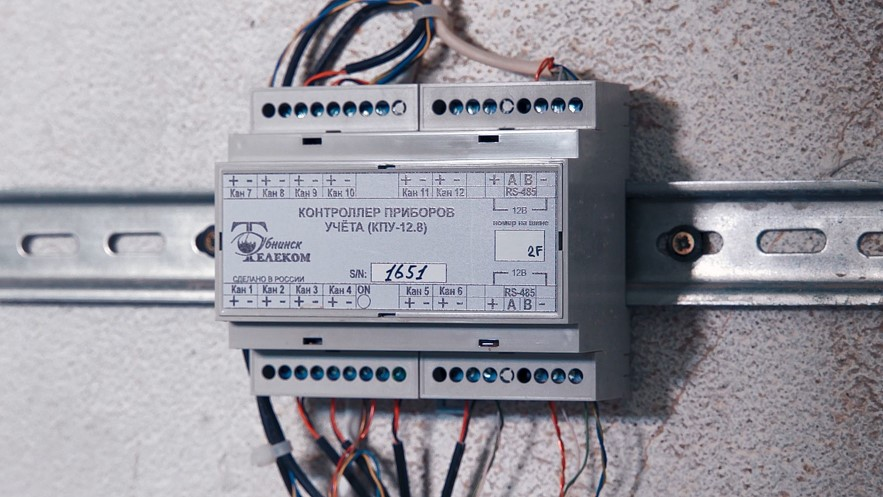
\includegraphics[width=0.7\linewidth]{pics/kpu}
	\caption{Контроллер приборов учета}
	\label{fig:kpu}
\end{figure}

\begin{table}[H]
	\caption{Технические данные КПУ} \label{tab:tab1}
	\centering
	\begin{tabular}{|p{10cm}|p{5cm}|}
		\hline 
		Максимальное количество подключаемых приборов учета & 12 \\ 
		\hline 
		Максимальное количество КПУ на шине RS485 & 128 \\ 
		\hline 
		Максимальная длина линии связи между КПУ и прибором учета, м, не более & 50 \\ 
		\hline 
		Максимальная длина линии связи между КПУ и персональным компьютером, м, не более & 1200 \\ 
		\hline
		Количество проводов между КПУ и счетчиком & 2 \\
		\hline
		Количество проводов между КПУ и персональным компьютером & 4 \\
		\hline
		Минимальное время замкнутого/разомкнутого состояния контактов датчиков, мс & 20 \\
		\hline
		Максимальное время реакции КПУ на полученную команду, мс & 50 \\
		\hline
		Количество импульсов на единицу измерения & от 10 до 2500 (кратное 10) \\
		\hline
		Потребляемая мощность, Вт, не более & 0,4 \\
		\hline
		Ресурс энергонезависимой памяти, лет & 50 \\
		\hline
		Максимально возможное хранимое показание & 999999,9 \\
		\hline
		Габаритные размеры, мм, не более & 140 x 95 x 40 \\
		\hline
		Масса блоков, кг, не более & 0,15 \\
		\hline
		Интерфейс связи с персональным компьютером & RS-485 9600 бод, 1 стоп-бит, без бита контроля \\
		\hline
	\end{tabular} 
\\Источник: документация к КПУ	
\end{table}

\subsection{Датчики}

Данные счётчики получили высокое распространение и были выбраны для использования благодаря простоте установки, малой погрешности и невысокой стоимости. 

\subsubsection{Itelma}

Счетчики Itelma для горячей и холодной воды (Рисунок~\ref{fig:itelma}). 

Счетчики на воду Ителма относятся к устройствам крыльчатого вида с механическим индикатором. Они сделаны на российских предприятиях по лицензии фирмы Siemens. Приборы изготавливают из комплектующих деталей немецкого производства. Это обеспечивает надежность и долговечность. \cite{itelma}

Устройства отличаются высокой чувствительностью, они работают при небольшом расходе воды, от 10 литров в час. Работают при давлении до 1 Мпа, диапазон температур составляет от 5 до 30 градусов для холодной воды, от 5 до 90 градусов – для горячей жидкости.

Счетчик воды WFK 24 дополнительно комплектуется импульсным датчиком с последовательным и шунтирующим (короткозамкнутым) сопротивлениями, соответствующими схеме НАМУР (NAMUR) для дистанционной передачи низкочастотных импульсов с контролем обрыва линии. \cite{saures}
Цена импульса – 0,01 м$^{3}$/имп. 

Счетчики защищены от манипулирования показаниями с помощью внешнего магнитного поля. Срок службы прибора для горячей воды составляет четыре года, для холодной воды --- шесть лет.

\begin{figure}[H]
	\centering
	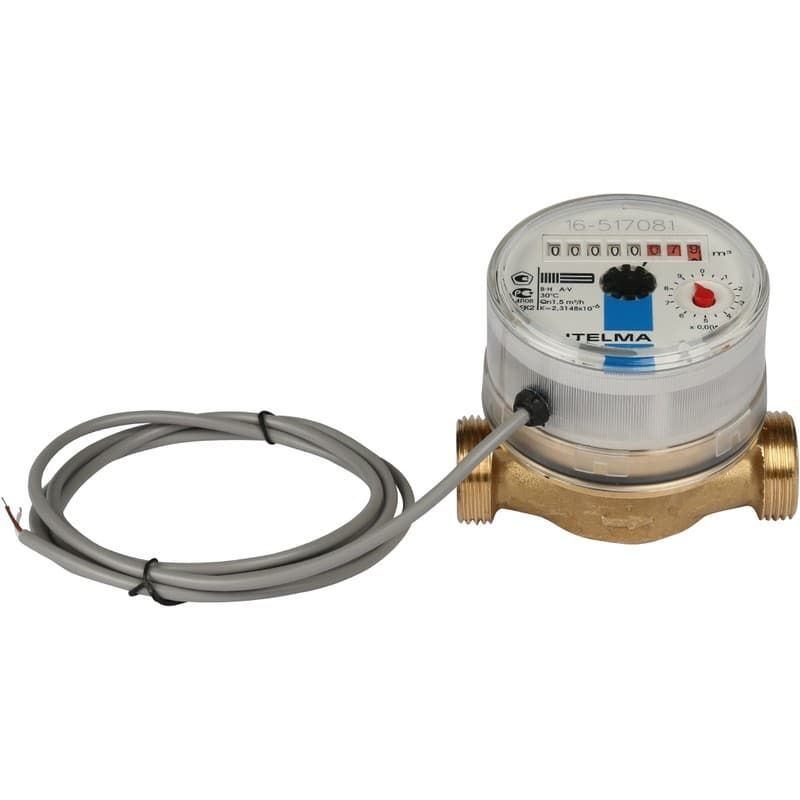
\includegraphics[width=0.5\linewidth]{pics/itelma}
	\caption{Внешний вид датчиков ITELMA}
	\label{fig:itelma}
\end{figure}

\subsubsection{SANEXT Mono}

Квартирные теплосчетчики предназначены для измерения количества потребляемой энергии в закрытых системах водяного отопления индивидуальных потребителей (поквартирный учет). Применяются при горизонтальной двухтрубной разводке системы отопления (Рисунок~\ref{fig:sanext}).

Принцип работы квартирного теплосчетчика основан на измерении расхода теплоносителя и разницы температур в подающем и обратном трубопроводах системы теплоснабжения и последующем определении количества потребленной энергии путем обработки результатов измерения вычислителем. \cite{sanext}
Преимущества механических теплосчетчиков SANEXT:

\begin{itemize}
	\item Минимальная монтажная высота, дает возможность установки теплосчетчика в небольших коллекторных шкаф или стеснённых условиях;
	\item Выносной дисплей упрощает процесс снятия показаний;
	\item Квартирные теплосчетчики с низким минимальным расход Qi от 5 л/ч подходит даже для помещений с малой площадью;
	\item Низкая потеря давления;
	\item Удобная навигация по меню счетчика;
	\item В архиве данных счётчика сохраняются ежемесячные показания счётчика в течение всего срока эксплуатации;
	\item Монтажные элементы выполнены из латуни, что обеспечивает длительный срок службы всех элементов приборов;
	\item Использование квартирных теплосчетчиков позволяет существенно экономить расход тепловой энергии;
	\item Межпроверочный интервал 6 лет;
\end{itemize}

Теплосчетчики включают в себя преобразователь расхода, вычислитель и пару платиновых термопреобразователей сопротивления.
Принцип работы теплосчетчиков состоит в измерении объема и температуры теплоносителя в подающем и обратном трубопроводах и последующем определении тепловой энергии, путем обработки результатов измерений вычислителем.

\begin{figure}[H]
	\centering
	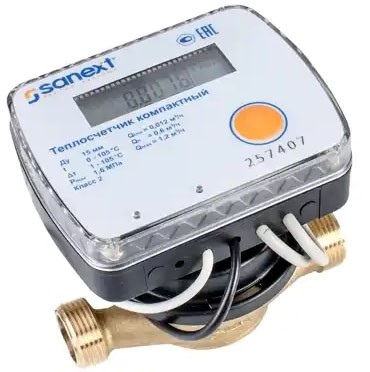
\includegraphics[width=0.4\linewidth]{pics/SANEXT}
	\caption{Внешний вид датчика SANEXT Mono}
	\label{fig:sanext}
\end{figure}

\subsubsection{Меркурий 201.5}

Счетчики ватт-часов активной энергии переменного тока электронные Меркурий 201, непосредственного включения, однофазные, однотарифные, с импульсным выходом, предназначены для измерения и учета электрической активной энергии в двухпроводных сетях переменного тока напряжением 230 В, частотой (50+-1) Гц. (Рисунок~\ref{fig:mercuriy})

Принцип действия счетчиков ватт-часов активной энергии переменного тока электронных «Меркурий 201» основан на учете информации, получаемой с импульсного выхода измерительной микросхемы. В качестве датчиков тока в счетчиках используется шунт, включенный последовательно в цепь тока. В качестве датчиков напряжения используются резистивные делители, включенные в параллельную цепь напряжения. \cite{incotexcom}

В качестве счетного механизма счетчики имеют электромеханические устройства отсчетные (УО) или жидкокристаллические индикаторы (ЖКИ) согласно таблице 1.

Счетчики с УО обеспечивают отображение информации в виде шестиразрядных чисел, пять старших разрядов дают показания в кВт-ч, шестой разряд, отделенный запятой, индицирует значение электроэнергии в десятых и сотых долях кВт-ч.

Счетчики с ЖКИ обеспечивают отображение энергопотребления нарастающим итогом в виде восьмиразрядных чисел, шесть старших разрядов дают показания в кВт-ч, два младших -указывают десятые и сотые доли кВт ч. Имеют световую индикацию мощности потребления. Период мерцания светового индикатора пропорционален уровню энергопотребления. В качестве испытательного выходного устройства счетчики имеют электрический и (или) оптический импульсный выход. Могут применяться автономно или в автоматизированных системах по сбору и учету информации о потребленной электроэнергии.  

\begin{figure}[H]
	\centering
	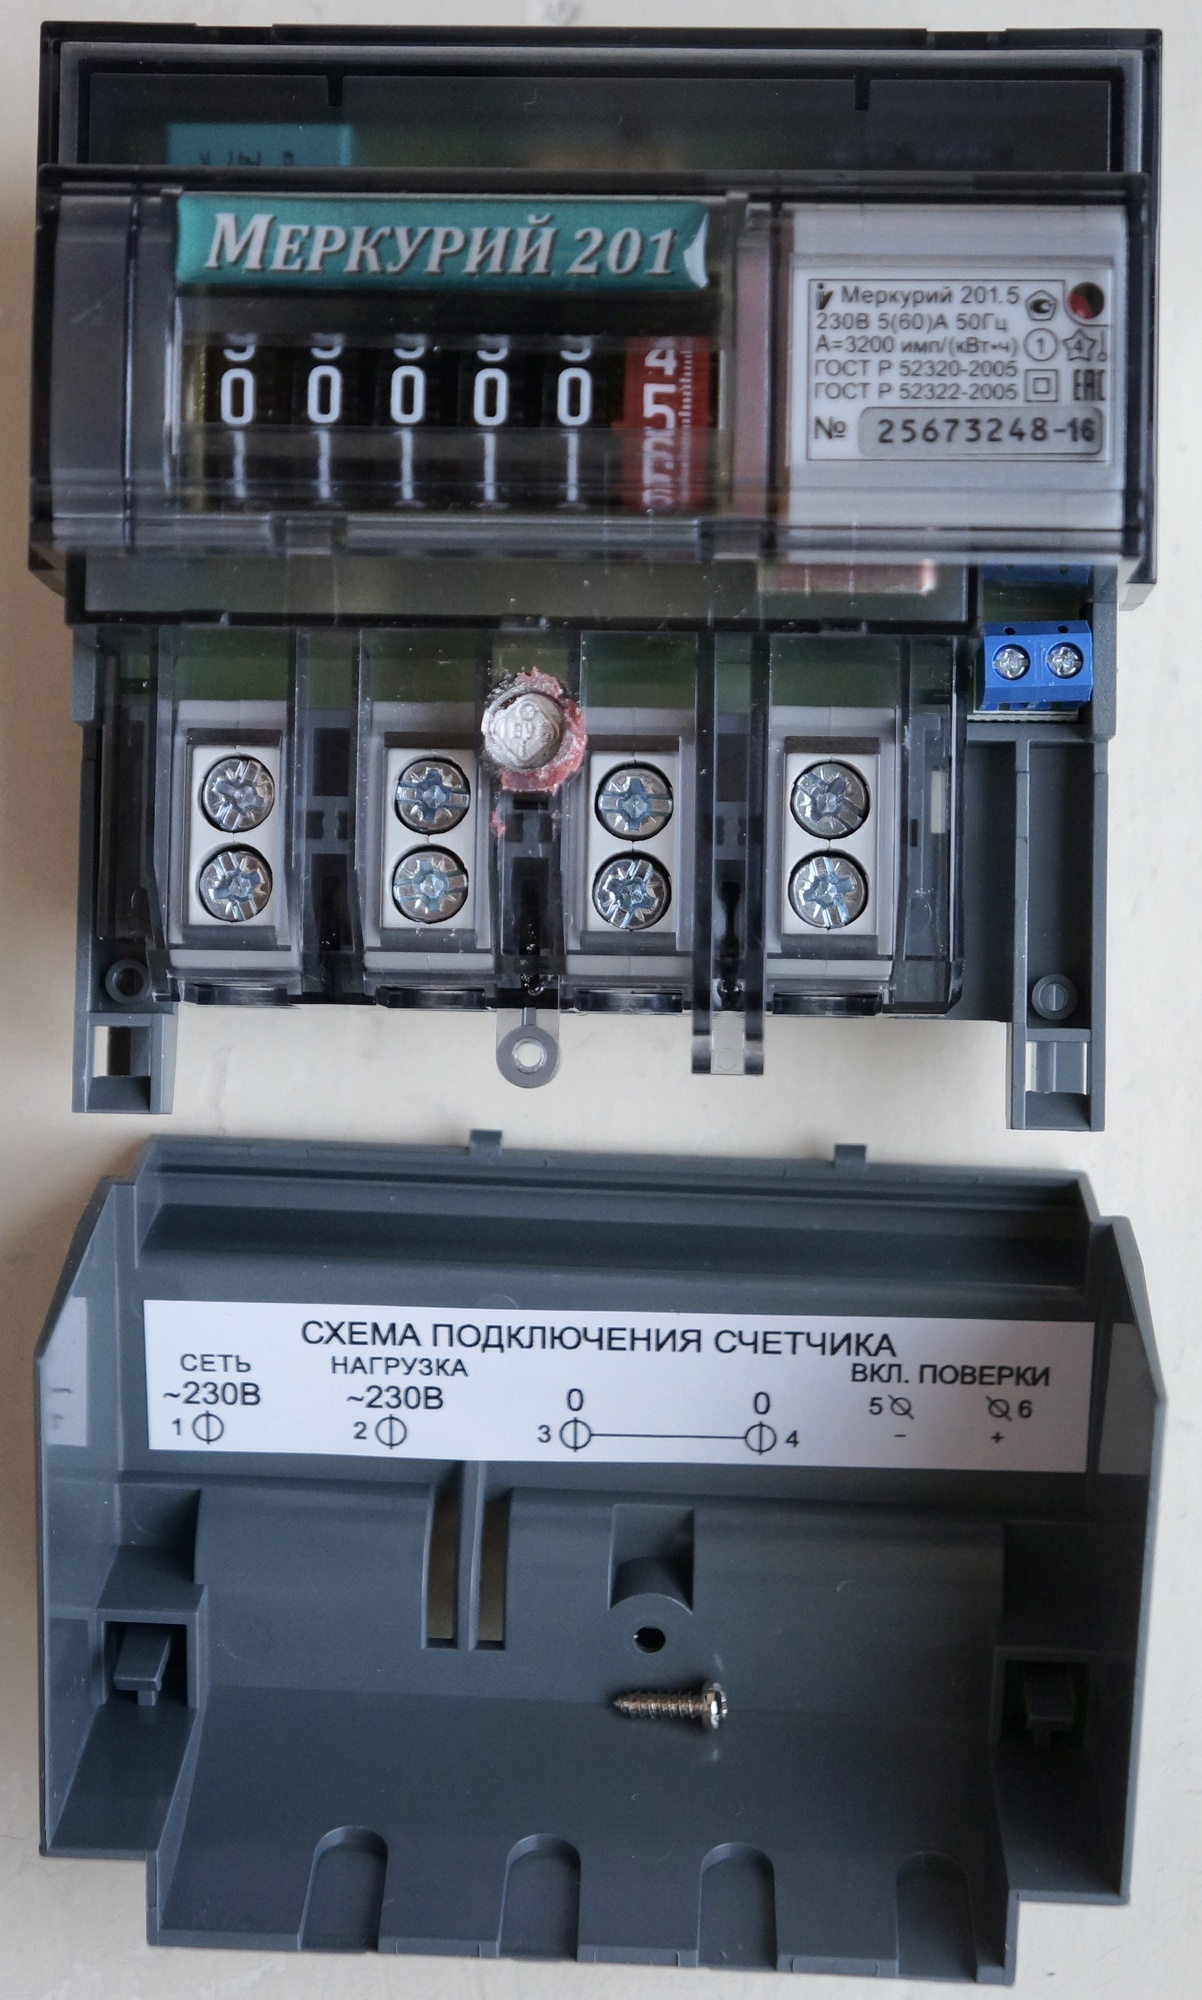
\includegraphics[width=0.5\linewidth]{pics/mercuriy}
	\caption{Меркурий 201.5}
	\label{fig:mercuriy}
\end{figure}